%%%%%%%%%%%%
%
% $Autor: Wings $
% $Datum: 2019-03-05 08:03:15Z $
% $Pfad: SetUp.tex $
% $Version: 4250 $
% !TeX spellcheck = en_GB/de_DE
% !TeX encoding = utf8
% !TeX root = manual 
% !TeX TXS-program:bibliography = txs:///biber
%
%%%%%%%%%%%%

\chapter{Inbetriebnahme}
Da Ihr Radarsystem bereits fertig montiert ist, sind nur wenige Handgriffe für den Start nötig.

\section{Aufstellung}
Platzieren Sie das Radarsystem auf einer ebenen Fläche (z. B. einem Tisch). Achten Sie darauf, dass sich im Umkreis von mindestens 50 cm keine Gegenstände befinden, die die Rotation der Dreheinheit behindern könnten.

\section{Software-Start}

Das Radarsystem wird in Kombination mit einer PC-Software betrieben, die als grafische Benutzeroberfläche (GUI) dient und die Sensordaten visualisiert. 

\subsection*{Schritt 1: Software installieren}
Um die Software zu beziehen, benötigen Sie lediglich den mitgelieferten USB-Stick mit der Benutzeroberfläche Anwendung.

\begin{itemize}
	\item Stecken sie den USB-Stick in den USB-A Eingang ihres Computers.
	\item Navigieren Sie über ihren Explorer zum USB-Stick. Laden Sie dort passend für ihr Betriebssystem die Software: \\
	\texttt{Benutzeroberflaeche-Ultraschallradar} herunter.
	\item Speichern Sie die heruntergeladene Anwendung an einen beliebigen Ort auf Ihrer lokalen Festplatte (z.\,B. auf den Desktop).
	
	\item \textbf{Hinweis:} Es ist keine Installation von Drittsoftware oder einer Entwicklungsumgebung  notwendig. Das Programm ist sofort lauffähig.
\end{itemize}

\subsection*{Schritt 2: Programm starten}
Um eine reibungslose Kommunikation zwischen Hardware und Software zu gewährleisten, halten Sie bitte folgende Reihenfolge ein:

\begin{enumerate}
	\item \textbf{Hardware anschlie\ss en:} Stellen Sie sicher, dass das Radarsystem über das Micro-USB Kabel mit dem Computer verbunden ist und mit Strom versorgt wird.
	
	\item \textbf{Software ausführen:} Navigieren Sie in den zuvor kopierten Ordner auf Ihrem Computer. Führen Sie die ausführbare Programmdatei: Benutzeroberflaeche-Ultraschallradar mit einem Doppelklick aus.
	
	\item \textbf{System-Initialisierung:} Die Benutzeroberfläche öffnet sich nun automatisch und das System fährt hoch und leitet den Hardware-Selbsttest ein.
\end{enumerate}

\subsection{Visuelle Darstellung:} 
Der Bildschirm auf dem Computermonitor ist abgedunkelt. Im Zentrum erscheint die Meldung: \textit{,,System fährt hoch... Hardware-Selbsttest wird durchgeführt.''}

\begin{figure}[htbp]
	\centering
	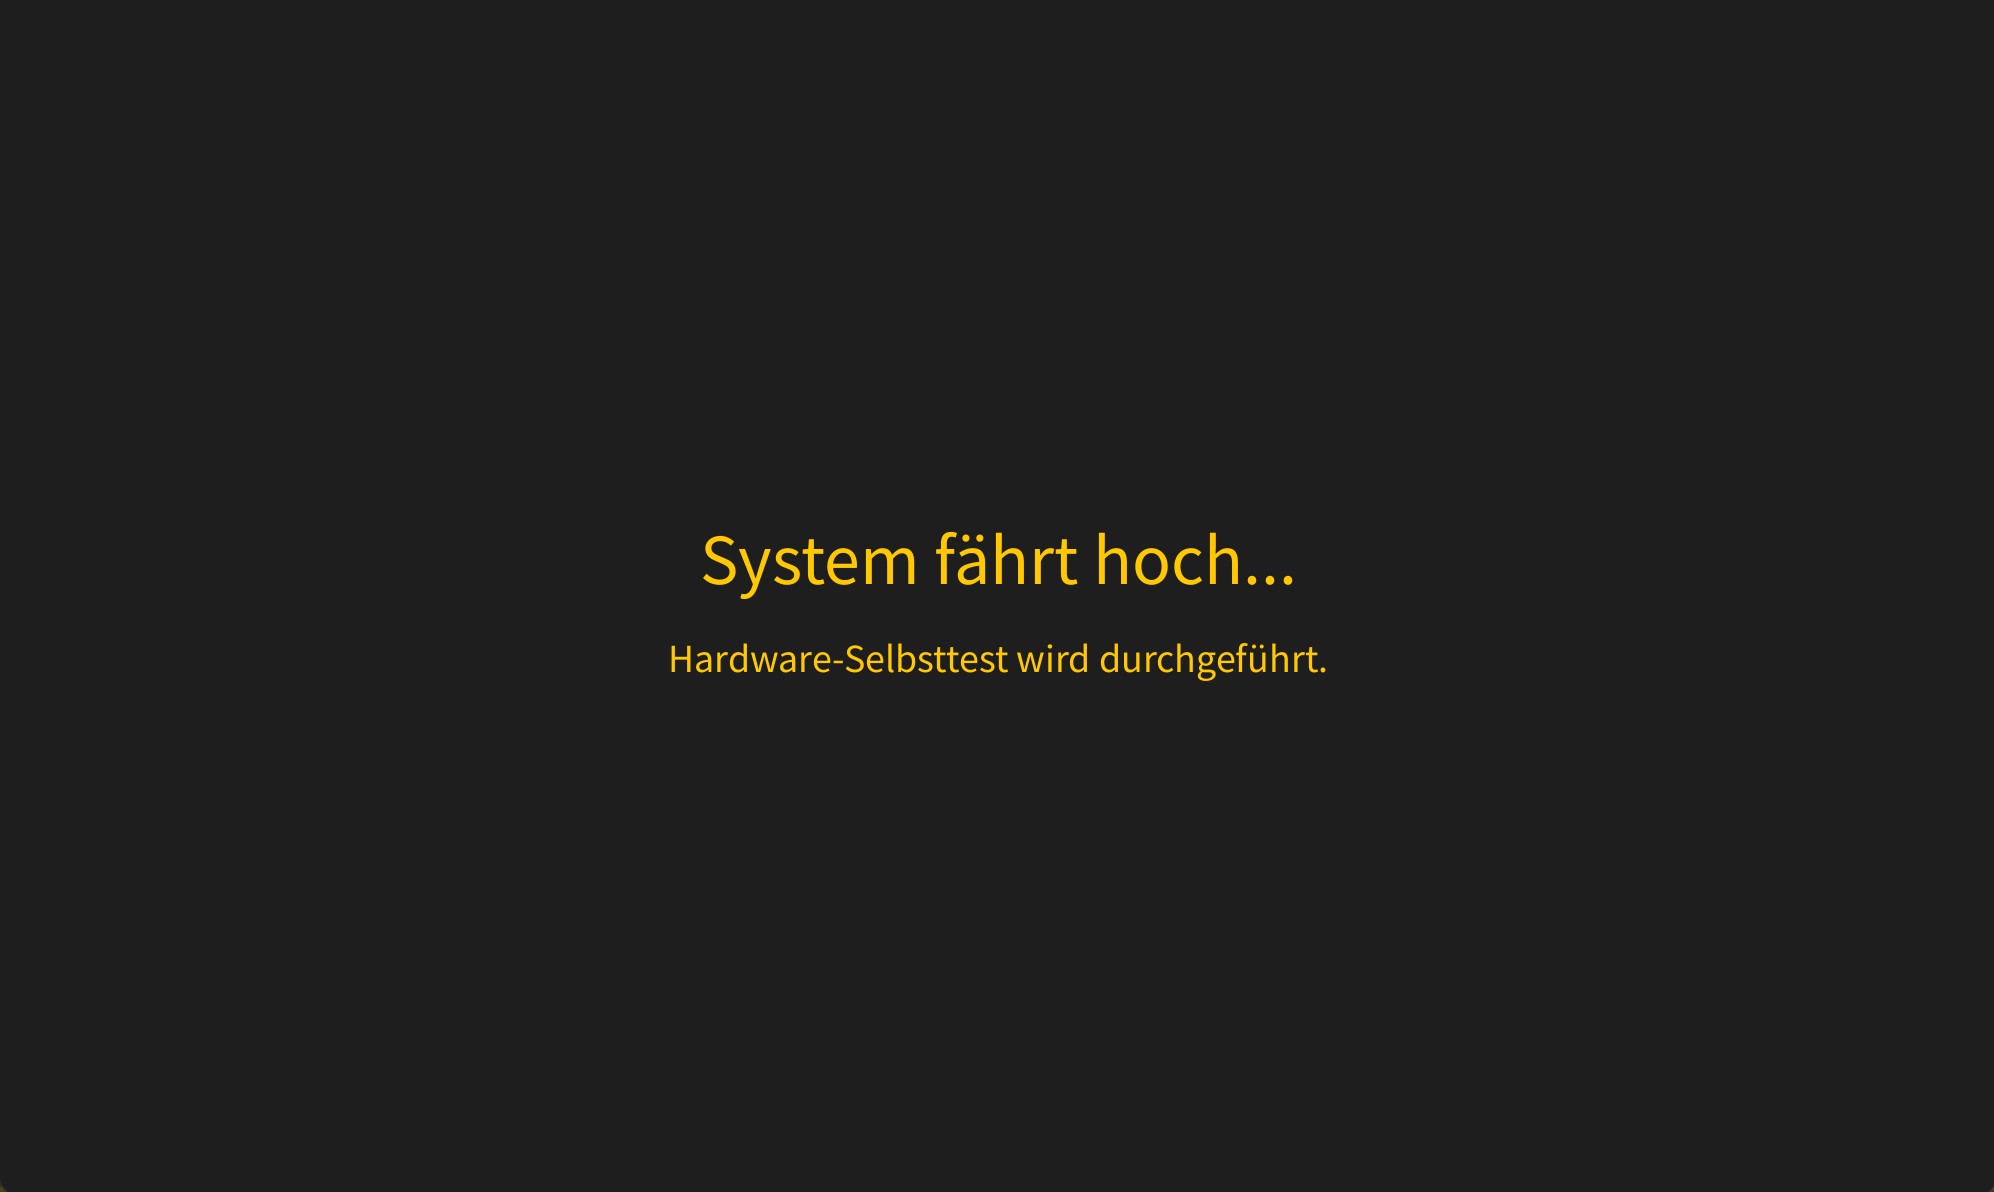
\includegraphics[width=0.8\textwidth]{General/BenutzeroberflaecheBilder/BenutzeroberflaecheSystemFaehrtHoch}
	\caption{Benutzeroberfläche: System fährt hoch}
	\label{fig: Benutzeroberfläche: System fährt hoch}
\end{figure}

\subsection{Bedeutung für den Anwender:} 
Das Radarsystem prüft die interne  Kommunikation, fährt die Dreheinheit in die definierte Ausgangsposition ($0^\circ$) und sendet einen ersten Test-Ultraschallimpuls, um Hardware- oder Kabelbrüche auszuschlie\ss en. Der Benutzer muss in dieser Phase keine Eingaben tätigen, sondern lediglich warten. Am Gehäuse der Hardware leuchten zur visuellen Bestätigung kurz beide LEDs (Grün und Rot) auf.